\providecommand{\curso}{Octavo Básico}
\providecommand{\colegio}{Colegio Divina Pastora}
\providecommand{\tituloDocumento}{Guía}
\providecommand{\subtituloDocumento}{Diagramas de caja}


\documentclass{cdplf-prueba}
\usetikzlibrary{fit,shapes.geometric}

\begin{document}

%% guia tabla 7b: 001
Utilice los datos de la tabla de frecuencia a continuación para completar el diagrama de caja.
\begin{center}\begin{tblr}{colspec={ccccc},hlines,vlines,hline{2,Z} = {1}{-}{},hline{2,Z} = {2}{-}{},row{even}={black!10},rowsep=0pt}
    .&Frecuencia&Probabilidad&Frecuencia Acumulada&Probabilidad Acumulada \\
   2&2&0.05&2&0.05 \\
   3&1&0.025&3&0.075 \\
   4&7&0.175&10&0.25 \\
   5&4&0.1&14&0.35 \\
   6&5&0.125&19&0.475 \\
   7&2&0.05&21&0.525 \\
   8&4&0.1&25&0.625 \\
   9&4&0.1&29&0.725 \\
   10&5&0.125&34&0.85 \\
   11&2&0.05&36&0.9 \\
   12&1&0.025&37&0.925 \\
   13&1&0.025&38&0.95 \\
   14&2&0.05&40&1 \\
\end{tblr}\end{center}

\begin{center}
\begin{tikzpicture}[ampersand replacement=\&,line width=1pt,x=1.5cm]
    \draw[<->] (-5.5,0) -- (5.5,0);
    \draw[] (-4,1.25) -- (-4,1.75) (-2,1) -- (-2,2) (2,1) -- (2,2) (4,1.25) -- (4,1.75)%
        (-4,1.5) -- (-2,1.5) (2,1.5) -- (4,1.5) (-2,2) -- (2,2) (-2,1) -- (2,1);
    \node[draw,dotted,rounded corners,inner sep=15pt,text width=25pt,anchor=north,yshift=-5pt] at (-4,0) {};
    \node[draw,dotted,rounded corners,inner sep=15pt,text width=25pt,anchor=north,yshift=-5pt,label=below:Primer cuartil $\left(Q_1\right)$] at (-2,0) {};
    \node[draw,dotted,rounded corners,inner sep=15pt,text width=25pt,anchor=north,yshift=-5pt,label=below:Tercer cuartil $\left(Q_3\right)$] at (2,0) {};
    \node[draw,dotted,rounded corners,inner sep=15pt,text width=25pt,anchor=north,yshift=-5pt] at (4,0) {};
    \draw[decorate, decoration={calligraphic brace,raise=0pt,amplitude=10pt},yshift=10pt] (-2,2) -- (2,2);
    \node[draw,dotted,rounded corners,inner sep=15pt,text width=25pt,anchor=north,yshift=55pt,label=above:Distancia inter-cuartil (DIQ)] at (0,2) {};
    \node[draw,dotted,rounded corners,inner sep=15pt,text width=25pt,anchor=north,yshift=-5pt,label=below:$Q_1 - 1.5\cdot\textrm{DIQ}$] (A) at (-4,-4) {};
    \node[draw,dotted,rounded corners,inner sep=15pt,text width=25pt,anchor=north,yshift=-5pt,label=below:Mínimo] (B) at (-4,-6) {};
    \node[draw,dashed,rounded corners,inner sep=20pt,yshift=-7pt,fit=(A) (B)] (C) {};
    \draw[->,dashed,shorten <=5pt] (C) -- (-4,-1.5) node [pos=0.5,anchor=west,text width=3cm] {El más grande de los dos};
    \node[draw,dotted,rounded corners,inner sep=15pt,text width=25pt,anchor=north,yshift=-5pt,label=below:$Q_3 + 1.5\cdot\textrm{DIQ}$] (D) at (4,-4) {};
    \node[draw,dotted,rounded corners,inner sep=15pt,text width=25pt,anchor=north,yshift=-5pt,label=below:Máximo] (E) at (4,-6) {};
    \node[draw,dashed,rounded corners,inner sep=20pt,yshift=-7pt,fit=(D) (E)] (F) {};
    \draw[->,dashed,shorten <=5pt] (F) -- (4,-1.5) node [pos=0.5,anchor=west,text width=3cm] {El más chico de los dos};
\end{tikzpicture}
\end{center}

\section*{Ejercicios}

\begin{ejercicios}
    \task! 
    %% 002
    \begin{center}\begin{tblr}{colspec={ccccc},hlines,vlines,hline{2,Z} = {1}{-}{},hline{2,Z} = {2}{-}{},row{even}={black!10},rowsep=0pt}
        .&Frecuencia&Probabilidad&Frecuencia Acumulada&Probabilidad Acumulada \\
       1&2&0.05&2&0.05 \\
       2&1&0.025&3&0.075 \\
       3&3&0.075&6&0.15 \\
       4&6&0.15&12&0.3 \\
       5&2&0.05&14&0.35 \\
       6&5&0.125&19&0.475 \\
       7&2&0.05&21&0.525 \\
       8&6&0.15&27&0.675 \\
       9&6&0.15&33&0.825 \\
       10&3&0.075&36&0.9 \\
       11&1&0.025&37&0.925 \\
       12&2&0.05&39&0.975 \\
       13&1&0.025&40&1 \\
    \end{tblr}\end{center}
    \vspace*{10pt}
    \begin{center}
    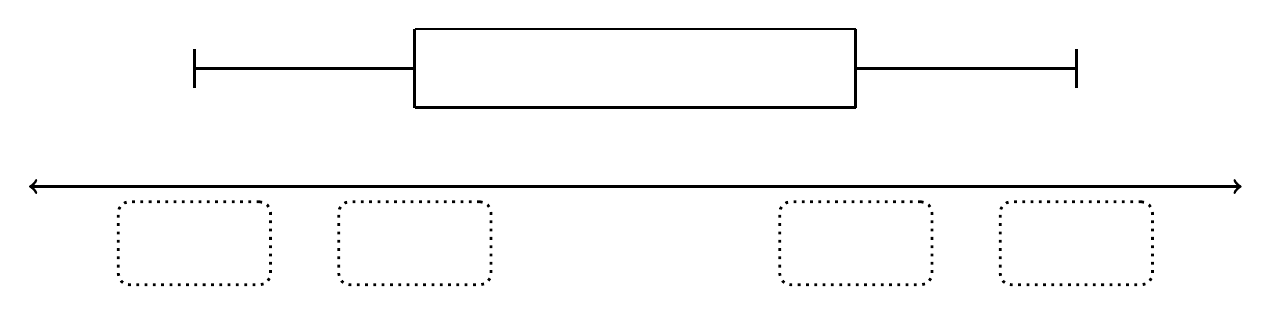
\begin{tikzpicture}[ampersand replacement=\&,line width=1pt,x=1.4cm]
        \draw[<->] (-5.5,0) -- (5.5,0);
        \draw[] (-4,1.25) -- (-4,1.75) (-2,1) -- (-2,2) (2,1) -- (2,2) (4,1.25) -- (4,1.75)%
            (-4,1.5) -- (-2,1.5) (2,1.5) -- (4,1.5) (-2,2) -- (2,2) (-2,1) -- (2,1);
        \node[draw,dotted,rounded corners,inner sep=15pt,text width=25pt,anchor=north,yshift=-5pt] at (-4,0) {};
        \node[draw,dotted,rounded corners,inner sep=15pt,text width=25pt,anchor=north,yshift=-5pt] at (-2,0) {};
        \node[draw,dotted,rounded corners,inner sep=15pt,text width=25pt,anchor=north,yshift=-5pt] at (2,0) {};
        \node[draw,dotted,rounded corners,inner sep=15pt,text width=25pt,anchor=north,yshift=-5pt] at (4,0) {};
    \end{tikzpicture}
    \end{center}
    %
    %     r$> dt
    %     [1] 14 10  4 13 13 14 11 10  4 11 14  9 14 11 10  9 11  7  8  9
    %
    %    r$> dt %>% tabyl %>% mutate(n_cum = cumsum(n), p_cum = cumsum(percent))
    %      . n percent n_cum p_cum
    %      4 2    0.10     2  0.10
    %      7 1    0.05     3  0.15
    %      8 1    0.05     4  0.20
    %      9 3    0.15     7  0.35
    %     10 3    0.15    10  0.50
    %     11 4    0.20    14  0.70
    %     13 2    0.10    16  0.80
    %     14 4    0.20    20  1.00
    %
    \task!
    \underline{Datos:} 14 \textbullet\hspace*{2pt}10 \textbullet\hspace*{2pt}4 \textbullet\hspace*{2pt}13 \textbullet\hspace*{2pt}13 \textbullet\hspace*{2pt}14 \textbullet\hspace*{2pt}11 \textbullet\hspace*{2pt}10 \textbullet\hspace*{2pt}4 \textbullet\hspace*{2pt}11 \textbullet\hspace*{2pt}14 \textbullet\hspace*{2pt}9 \textbullet\hspace*{2pt}14 \textbullet\hspace*{2pt}11 \textbullet\hspace*{2pt}10 \textbullet\hspace*{2pt}9 \textbullet\hspace*{2pt}11 \textbullet\hspace*{2pt}7 \textbullet\hspace*{2pt}8 \textbullet\hspace*{2pt}9
    \vspace{10pt}
    \begin{desarrollo}[height=5cm]
    \end{desarrollo}
    \vspace{10pt}
    \begin{center}
        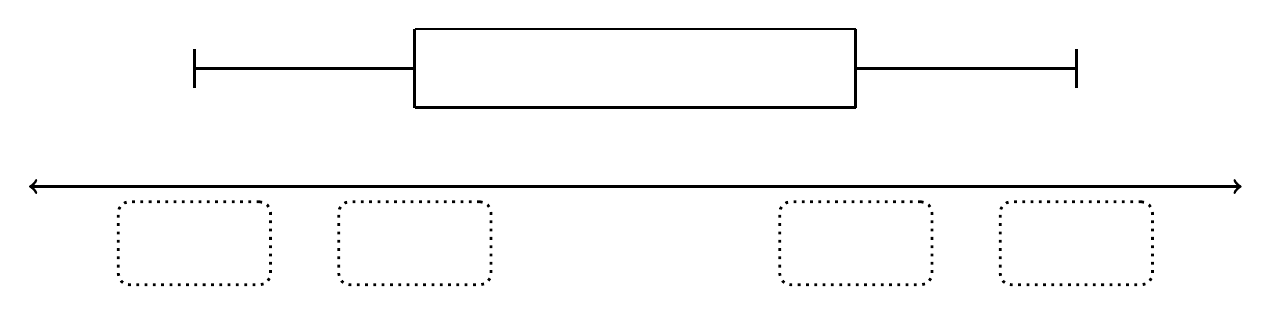
\begin{tikzpicture}[ampersand replacement=\&,line width=1pt,x=1.4cm]
            \draw[<->] (-5.5,0) -- (5.5,0);
            \draw[] (-4,1.25) -- (-4,1.75) (-2,1) -- (-2,2) (2,1) -- (2,2) (4,1.25) -- (4,1.75)%
                (-4,1.5) -- (-2,1.5) (2,1.5) -- (4,1.5) (-2,2) -- (2,2) (-2,1) -- (2,1);
            \node[draw,dotted,rounded corners,inner sep=15pt,text width=25pt,anchor=north,yshift=-5pt] at (-4,0) {};
            \node[draw,dotted,rounded corners,inner sep=15pt,text width=25pt,anchor=north,yshift=-5pt] at (-2,0) {};
            \node[draw,dotted,rounded corners,inner sep=15pt,text width=25pt,anchor=north,yshift=-5pt] at (2,0) {};
            \node[draw,dotted,rounded corners,inner sep=15pt,text width=25pt,anchor=north,yshift=-5pt] at (4,0) {};
        \end{tikzpicture}
        \end{center}
\end{ejercicios}

   
\end{document}